\section*{静电场}

\subsubsection*{一. 选择题}

1. 一均匀带电球面,电荷面密度为$\sigma$,球面内电场强度处处为零,球面上面元$\d S$带有$\sigma\d S$的电荷,该电荷在球面内各点产生的电场强度\fbox{处处不为零}.

2. 下列说法中正确的是\fbox{(C)}.\pp
    (C) 场强可由$\vec{E}=\vec{F}/q$定出,其中$q$为试验电荷可负可正,$\vec{F}$为试验电荷所受的电场力.

4. 将一个试验电荷$q_0$(正电荷)放在带有负电荷的大导体附近$P$点处(如图),测得它所受的力为$F$.若考虑到电荷$q_0$不是足够小,则\fbox{(B)}.\pp
    (B) $F/q_0$比$P$点处原先的场强数值小.

图4.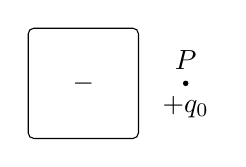
\begin{tikzpicture}
\draw[rounded corners=2pt] (0,0) rectangle (1.4,1.4);
\draw (0.7,0.7) node {$-$};
\fill (2,0.7) circle (1pt);
\draw (2,1) node {$P$};
\draw (2,0.4) node {$+q_0$};
\end{tikzpicture}
图7.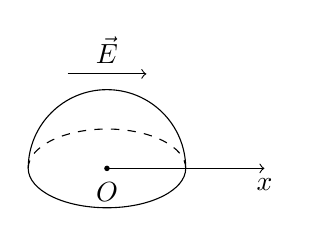
\begin{tikzpicture}
\draw (0,0) arc [start angle=0, end angle=180, x radius=1, y radius=1];
\draw[dashed] (0,0) arc [start angle=0, end angle=180, x radius=1, y radius=0.5];
\draw (0,0) arc [start angle=360, end angle=180, x radius=1, y radius=0.5];
\draw[->] (-1.5,1.2) -- (-0.5,1.2);
\draw (-1,1.5) node {$\vec E$};
\fill (-1,0) circle (1pt);
\draw (-1,-0.3) node {$O$};
\draw[->] (-1,0) -- (1,0);
\draw (1,-0.2) node {$x$};
\end{tikzpicture}
图8.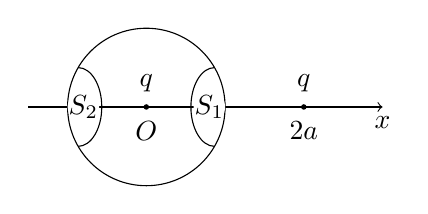
\begin{tikzpicture}
\draw (0,0) circle (1);
\fill (0,0) circle (1pt);
\draw (0,0.3) node {$q$};
\draw (0,-0.3) node {$O$};
\draw[->] (-1.5,0) -- (3,0);
\draw (3,-0.2) node {$x$};
\fill (2,0) circle (1pt);
\draw (2,0.3) node {$q$};
\draw (2,-0.3) node {$2a$};
\draw (30:1) arc [start angle=90, delta angle=180, y radius=0.5, x radius=0.3];
\fill[white] (0.8,0) circle (0.2);
\draw (0.8,0) node {$S_1$};
\draw (210:1) arc [start angle=270, delta angle=180, y radius=0.5, x radius=0.3];
\fill[white] (-0.8,0) circle (0.2);
\draw (-0.8,0) node {$S_2$};
\end{tikzpicture}

7. 一电场强度为$\vec E$的均匀电场,$\vec E$的方向沿$x$轴正方向,如图,则通过图中一半径为$R$的半球面的电场强度通量为\fbox{0}.

8. 有两个电荷都是$+q$的点电荷,相距为$2a$.今以左边的点电荷所在处为球心,以$a$为半径作一球形高斯面.在球面上取两块相等的小面积$S_1$和$S_2$,其位置如图所示.设通过$S_1$和$S_2$的电场强度通量分别为$\varPhi_1$和$\varPhi_2$,通过整个球面的电场强度通量为$\varPhi_S$,则\fbox{$\varPhi_1<\varPhi_2, \varPhi_S=q/\varepsilon_0$}.

9. 如图所示,一个电荷为$q$的点电荷位于立方体的$A$角上,则通过侧面$abcd$的电场强度通量等于\fbox{$\frac{q}{24\varepsilon_0}$}.

图9.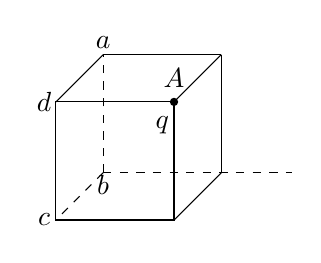
\begin{tikzpicture}[scale=1.5]
\draw (0,0) rectangle (1,1);
\draw[dashed] (0.4,0.4) -- (0.4,1.4);
\draw[dashed] (0.4,0.4) -- (2,0.4);
\draw[dashed] (0.4,0.4) -- (0,0);
\draw (0,1) -- (0.4,1.4);
\draw (1,1) -- (1.4,1.4);
\draw (1,0) -- (1.4,0.4);
\draw (0.4,1.4) -- (1.4,1.4);
\draw (1.4,0.4) -- (1.4,1.4);
\draw (-0.1,0) node {$c$};
\draw (-0.1,1) node {$d$};
\draw (0.4,1.5) node {$a$};
\draw (0.4,0.3) node {$b$};
\fill (1,1) circle (1pt);
\draw (1,1.2) node {$A$};
\draw (0.9,0.8) node {$q$};
\end{tikzpicture}
图10.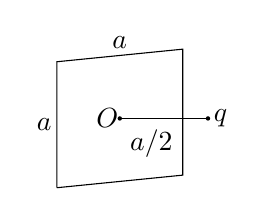
\begin{tikzpicture}[scale=0.8]
\draw (-1,-1) -- (-1,1) -- (1,1.2) -- (1,-0.8) -- (-1,-1);
\fill (0,0.1) circle (1pt);
\draw (-0.2,0.1) node {$O$};
\draw (0,0.1) -- (1.4,0.1);
\draw (0.5,-0.3) node {$a/2$};
\draw (-1.2,0) node {$a$};
\draw (0,1.3) node {$a$};
\fill (1.4,0.1) circle (1pt);
\draw (1.6,0.1) node {$q$};
\end{tikzpicture}
图16.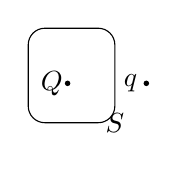
\begin{tikzpicture}
\draw[rounded corners=6pt] (0,0) rectangle (1.1,1.2);
\draw (1.1,0) node {$S$};
\fill (0.5,0.5) circle (1pt);
\draw (0.3,0.5) node {$Q$};
\fill (1.5,0.5) circle (1pt);
\draw (1.3,0.5) node {$q$};
\end{tikzpicture}

10. 有一边长为$a$的正方形平面,在其中垂线上距中心$O$点$a/2$处,有一电荷为$q$的正点电荷,如图所示,则通过该平面的电场强度通量为\fbox{$\frac{q}{6\varepsilon_0}$}.

11. 高斯定理$\oint_S\vec E\cdot\d\vec S=\int_V\rho\d V/\varepsilon_0$ \fbox{(A)}.\pp
    (A) 适用于任何静电场.

12. 关于高斯定理的理解有下面几种说法,其中正确的是\fbox{(D)}.\pp
    (D) 如果高斯面内有静电荷,则通过高斯面的电场强度通量必不为零.

15. 根据高斯定理的数学表达式$\oint_S\vec E\cdot\d\vec S=\sum q/\varepsilon_0$可知\fbox{(C)}.\pp
    (C) 闭合面内的电荷代数和为零时,闭合面上各点场强不一定处处为零.

16. 点电荷$Q$被曲面$S$所包围,从无限远处引入另一点电荷$q$至曲面外一点,如图所示,则引入前后\fbox{(D)}.\pp
    (D) 曲面$S$的电场强度通量不变,曲面上各点场强变化.

17. 半径为$R$的均匀带电球体的静电场中各点的电场强度大小$E$与距球心距离$r$的关系曲线为\fbox{(B)}.

图17.(B)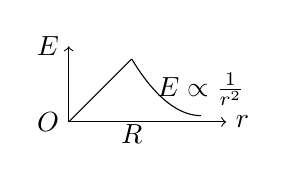
\begin{tikzpicture}[scale=0.8]
\draw (0,0) node[left] {$O$};
\draw[->] (0,0) -- (2.5,0) node[right] {$r$};
\draw[->] (0,0) -- (0,1.2) node[left] {$E$};
\draw (1,-0.2) node {$R$};
\draw (0,0) -- (1,1);
\draw (1,1) parabola[bend at end] (2.1,0.1) node[above] {$E\propto\D\frac{1}{r^2}$};
% \draw[dashed] (1,0) -- (1,1);
\end{tikzpicture}
图18.(B)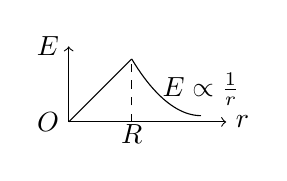
\begin{tikzpicture}[scale=0.8]
\draw (0,0) node[left] {$O$};
\draw[->] (0,0) -- (2.5,0) node[right] {$r$};
\draw[->] (0,0) -- (0,1.2) node[left] {$E$};
\draw (1,-0.2) node {$R$};
\draw (0,0) -- (1,1);
\draw (1,1) parabola[bend at end] (2.1,0.1) node[above] {$E\propto\D\frac{1}{r}$};
\draw[dashed] (1,0) -- (1,1);
\end{tikzpicture}

18. 半径为$R$的“无限长”均匀带电圆柱体的静电场中各点的电场强度大小$E$与距轴线距离$r$的关系曲线为\fbox{(B)}.

23. 有$N$个电荷均为$q$的点电荷,以两种方式分布在相同半径的圆周上:一种是无规则的分布,另一种是均匀分布.比较这两种情况下在过圆心$O$并垂直于圆平面的$z$轴上任一点$P$(如图所示)的场强与电势,则有\fbox{(C)}.\pp
    (C) 场强分量$E_z$相等,电势相等.

24. 静电场中某点电势的数值等于\fbox{(C)}.\pp
    (C) 单位正电荷置于该点时具有的电势能.

25. 关于静电场中某点电势值的正负,\fbox{(C)}.\pp
    (C) 电势值的正负取决于电势零点的选取.

26. 如图,在点电荷$q$的电场中,选取以$q$为中心、$R$为半径的球面上一点$P$处作电势零点,则与点电荷$q$距离为$r$的点$P'$电势为\fbox{$\frac{q}{4\pi\varepsilon_0}(\frac{1}{r}-\frac{1}{R})$}.

图23.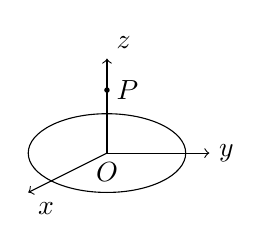
\begin{tikzpicture}
\draw (0,0) node[below] {$O$};
\draw[->] (0,0) -- (-1,-0.5) node[below right] {$x$};
\draw[->] (0,0) -- (1.3,0) node[right] {$y$};
\draw[->] (0,0) -- (0,1.2) node[above right] {$z$};
\fill (0,0.8) circle(1pt) node[right] {$P$};
\draw (0,0) ellipse[x radius=1,y radius=0.5];
\end{tikzpicture}
图26.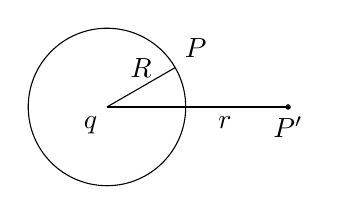
\begin{tikzpicture}
\draw (0,0) circle (1);
\draw (0,0) -- (30:1);
\draw (30:.5) node[above] {$R$};
\draw (30:1) node[above right] {$P$};
\draw (0,0) node[below left] {$q$};
\draw (0,0) -- (2.3,0);
\draw (1.5,0) node[below] {$r$};
\fill (2.3,0) circle (1pt);
\draw (2.3,0) node[below] {$P'$};
\end{tikzpicture}
图27.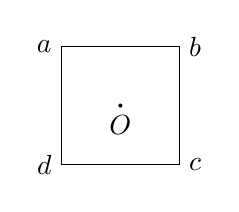
\begin{tikzpicture}[scale=1.5]
\draw (0,0) rectangle (1,1);
\draw (0,0) node[left] {$d$};
\draw (0,1) node[left] {$a$};
\draw (1,0) node[right] {$c$};
\draw (1,1) node[right] {$b$};
\fill (.5,.5) circle (.5pt) node[below] {$O$};
\end{tikzpicture}

27. 如图所示,边长为$l$的正方形,在其四个顶点上各放有等量的点电荷.若正方形中心$O$处的场强值和电势值都等于零,则\fbox{(C)}.\pp
    (C) 顶点$a,c$处是正电荷,$b,d$处是负电荷.

30. 如图所示,两个同心球壳.内球壳半径为$R_1$,均匀带有电荷$Q$;外球壳半径为$R_2$,壳的厚度忽略,原先不带电,但与地相连接.设地为电势零点,则在两球之间距离球心为$r$的点$P$处电场强度大小为\fbox{$E=\frac{Q}{4\pi\varepsilon_0r^2}$},电势为\fbox{$U=\frac{Q}{4\pi\varepsilon_0}(\frac{1}{r}-\frac{1}{R})$}.

图30.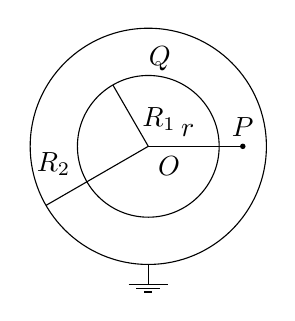
\begin{tikzpicture}[scale=0.5]
\draw (0,0) node[below right] {$O$};
\draw (0,0) circle (1.8);
\draw (0,0) circle (3);
\draw (0,0) -- (120:1.8);
\draw (120:0.8) node[right] {$R_1$};
\draw (80:1.7) node[above] {$Q$};
\draw (0,0) -- (210:3);
\draw (210:2) node[above left] {$R_2$};
\draw (0,0) -- (2.4,0);
\draw (1,0) node[above] {$r$};
\fill (2.4,0) circle (2pt);
\draw (2.4,0) node[above] {$P$};
\draw (0,-3) -- (0,-3.5);
\draw (-0.5,-3.5) -- (0.5,-3.5);
\draw (-0.3,-3.6) -- (0.3,-3.6);
\draw (-0.1,-3.7) -- (0.1,-3.7);
\end{tikzpicture}
图32.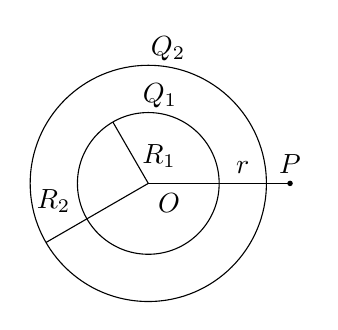
\begin{tikzpicture}[scale=0.5]
\draw (0,0) node[below right] {$O$};
\draw (0,0) circle (1.8);
\draw (0,0) circle (3);
\draw (0,0) -- (120:1.8);
\draw (120:0.8) node[right] {$R_1$};
\draw (80:1.7) node[above] {$Q_1$};
\draw (80:2.9) node[above] {$Q_2$};
\draw (0,0) -- (210:3);
\draw (210:2) node[above left] {$R_2$};
\draw (0,0) -- (3.6,0);
\draw (2.4,0) node[above] {$r$};
\fill (3.6,0) circle (2pt);
\draw (3.6,0) node[above] {$P$};
\end{tikzpicture}
图33.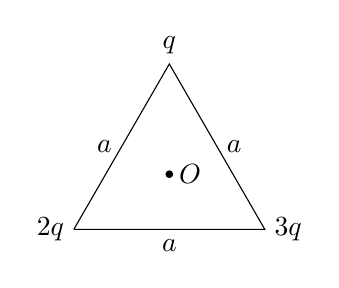
\begin{tikzpicture}[scale=1.4]
\draw (210:1) -- (90:1) -- (330:1) -- (210:1);
\fill (0,0) circle (1pt);
\draw (0,0) node[right] {$O$};
\draw (210:1) node[left] {$2q$};
\draw (90:1) node[above] {$q$};
\draw (330:1) node[right] {$3q$};
\draw (30:.5) node[right] {$a$};
\draw (150:.5) node[left] {$a$};
\draw (270:.5) node[below] {$a$};
\end{tikzpicture}

32. 如图所示,两个同心的均匀带电球面,内球面半径为$R_1$、带电荷$Q_1$,外球面半径为$R_2$、带电荷$Q_2$.设无穷远处为电势零点,则在外球面之外距离球心为$r$处的点$P$的电势$U$为\fbox{$\frac{Q_1+Q_2}{4\pi\varepsilon_0r}$}.

33. 如图所示,边长为$a$的等边三角形的三个顶点上,分别放置着三个正的点电荷$q,2q,3q$.若将另一正点电荷$Q$从无穷远处移到三角形中心$O$处,外力所做的功为\fbox{$\frac{3\sqrt{3}qQ}{2\pi\varepsilon_0a}$}.

34. 点电荷$-q$位于圆心$O$处,$A,B,C,D$为同一圆周上的四点,如图所示.现将一试验电荷从$A$点分别移动到$B,C,D$各点,则\fbox{(D)}.\pp
    (D) 从$A$到各点,电场力做功相等.

图34.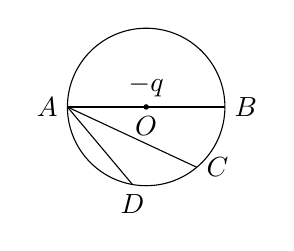
\begin{tikzpicture}
\draw (0,0) node[below] {$O$};
\draw (0,0) node[above] {$-q$};
\draw (0,0) circle (1);
\fill (0,0) circle (1pt);
\draw (-1,0) node[left] {$A$}
    -- (1,0) node[right] {$B$};
\draw (-1,0) -- (310:1) node[right] {$C$};
\draw (-1,0) -- (260:1) node[below] {$D$};
\end{tikzpicture}
图35.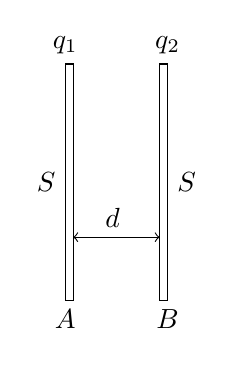
\begin{tikzpicture}
\draw (0,0) rectangle (.1,3);
\draw (1.2,0) rectangle (1.3,3);
\draw (0,1.5) node[left] {$S$};
\draw (0,3) node[above] {$q_1$};
\draw (0,0) node[below] {$A$};
\draw (1.3,1.5) node[right] {$S$};
\draw (1.3,0) node[below] {$B$};
\draw (1.3,3) node[above] {$q_2$};
\draw[<->] (0.1,0.8) -- (1.2,0.8);
\draw (0.6,0.8) node[above] {$d$};
\end{tikzpicture}
图36.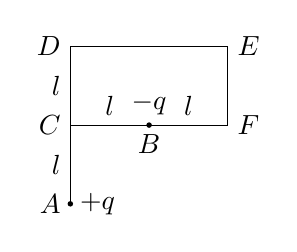
\begin{tikzpicture}
\draw (0,0) rectangle (2,1);
\draw (0,0) node[left] {$C$};
\draw (0,1) node[left] {$D$};
\draw (2,1) node[right] {$E$};
\draw (2,0) node[right] {$F$};
\draw (0,0) -- (0,-1) node[left] {$A$};
\fill (0,-1) circle (1pt) node[right] {$+q$};
\fill (1,0) circle (1pt);
\draw (1,0) node[below] {$B$};
\draw (1,0) node[above] {$-q$};
\draw (0,0.5) node[left] {$l$};
\draw (0,-0.5) node[left] {$l$};
\draw (0.5,0) node[above] {$l$};
\draw (1.5,0) node[above] {$l$};
\end{tikzpicture}

35. 两块面积均为$S$的金属平板$A$和$B$彼此平行放置,板间距离为$d$($d$远小于板的线度),设$A$板带有电荷$q_1$,$B$板带有电荷$q_2$,则$A,B$两板间的电势差$U_{AB}$为\fbox{$\frac{q_1-q_2}{2\varepsilon_0S}d$}.

36. 如图所示,$CDEF$为一矩形,边长分别为$l$和$2l$.在$DC$延长线上$CA=l$处的$A$点有点电荷$+q$,在$CF$的中点$B$有点电荷$-q$,若使单位正电荷从$C$点沿$CDEF$径运动到$F$点,则电场力所做的功等于\fbox{$\frac{q}{4\pi\varepsilon_0l}\cdot\frac{\sqrt5-1}{\sqrt5}$}.

37. 图中实线为某电场中的电场线,虚线表示等势(位)面,由图可以看出\fbox{(D)}.\pp
    (D) $E_A<E_B<E_C, U_A>U_B>UC$.

图37.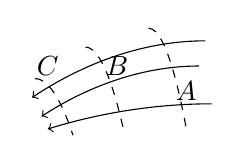
\begin{tikzpicture}[scale=0.8]
% \draw[help lines] (0,0) grid (3,2);
\draw[->] (3,0.4) parabola (0.4,0);
\draw[dashed] (2,1.6) parabola (2.6,0);
\draw (2.6,0.6) node {$A$};
\draw[->] (2.8,1) parabola (0.3,0.2);
\draw[dashed] (1,1.3) parabola (1.6,0);
\draw (1.5,1) node {$B$};
\draw[->] (2.9,1.4) parabola (0.15,0.5);
\draw[dashed] (0.2,0.8) parabola (0.8,-0.1);
\draw (0.4,1) node {$C$};
\end{tikzpicture}
图38.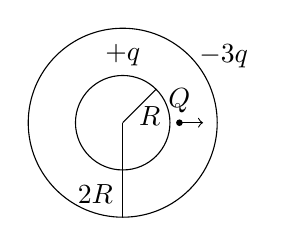
\begin{tikzpicture}[scale=0.6]
\draw (0,0) circle (1);
\draw (0,0) circle (2);
\draw (0,0) -- (45:1);
\draw (0,0) -- (270:2);
\draw (45:.2) node[right] {$R$};
\draw (270:1.5) node[left] {$2R$};
\fill (1.2,0) circle (2pt) node[above] {$Q$};
\draw[->] (1.2,0) -- (1.7,0);
\draw (90:1) node[above] {$+q$};
\draw (45:2) node[right] {$-3q$};
\end{tikzpicture}
图47.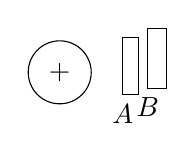
\begin{tikzpicture}[scale=0.4]
\draw (0,0) circle (1);
\draw (0,0) node {$+$};
\draw (2,-0.7) node[below] {$A$} rectangle (2.5,1.1);
\draw (2.8,-0.5) node[below] {$B$} rectangle (3.4,1.4);
\end{tikzpicture}
图48.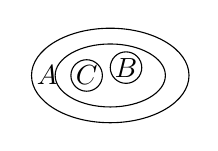
\begin{tikzpicture}
\draw (0,0) circle[x radius=1,y radius=0.6];
\draw (0,0) circle[x radius=0.7,y radius=0.4];
\draw (-0.3,0) node {$C$} circle (0.2);
\draw (0.2,0.1) node{$B$} circle (0.2);
\draw (-0.8,0) node {$A$};
\end{tikzpicture}

38. 如图所示,在真空中半径分别为$R$和$2R$的两个同心球面,其上分别均匀地带有电荷$+q$和$-3q$.今将一电荷为$+Q$的带电粒子从内球面处由静止释放,则该粒子到达外球面时的动能为\fbox{$\frac{Qq}{8\pi\varepsilon_0R}$}.

47. 把$A,B$两块不带电的导体放在一带正电导体的电场中,如图所示.设无限远处为电势零点,$A$的电势为$U_A$,$B$的电势为$U_B$,则\fbox{$U_B<U_A$}.

48. 如图所示,一封闭的导体壳$A$内有两个导体$B$和$C$.$A,C$不带电,$B$带正电,则$A,B,C$三导体的电势关系是\fbox{$U_B>U_C>U_A$}.

52. 一个平行板电容器,充电后与电源断开,当用绝缘手柄将电容器两极板间距拉大,则两级板间的电势差\fbox{$U_{12}$增大},电场强度大小\fbox{$E$不变},电场能量\fbox{$W$增大}.

\subsubsection*{二. 填空题}

\subsubsection*{三. 计算题}
